\documentclass{beamer}
\usetheme{Berkeley}
\usecolortheme{seahorse}
\usepackage{hyperref}
\usepackage{graphicx}
\usepackage{amsmath}
\def\bm#1{\mbox{\boldmath $#1$}}
\include{macros}
 
\title{Sampling forest plots using adaptive empirical cumulative distribution functions}
\author{John Tipton}
\date{\today}
\begin{document}
%
\begin{frame}
  \maketitle
\end{frame}
%
\begin{frame}
  \frametitle{Introduction}
  \section{Introduction}
  Goals
  \begin{itemize}
    \item Estimate plot level biomass with increased precision \vspace{3mm}
    \item Increase the number of large dbh trees in the sample \vspace{3mm}
    \item Easily implementable in the field
  \end{itemize}
\end{frame}
%
\begin{frame}
  \frametitle{Biomass Model}
  DBH is used as a predictor for biomass using an allometric equation.   Under simple random sampling, the model of interest is the allometric tree growth equation with exponential error given by 
  \begin{align}
  \label{1}
     Y_i & =  X_i^{\beta_1} e^{\beta_0 + \epsilon}
  \end{align}
  where $Y_i$ is biomass for tree $i$, $X_i$ is dbh for tree $i$, $\epsilon \sim N(0, \sigma^2)$ is a random error, and $\beta_0$ and $\beta_1$ are coefficients to be estimated.
\end{frame}
%
\begin{frame}
  \frametitle{The Model}
  A plot of the allometric relationship using simulated data is seen below
  \begin{figure}
    \centering
%     \caption{Plot of simulated allometric relationship typical of a sample plot (assumes one species only)}
    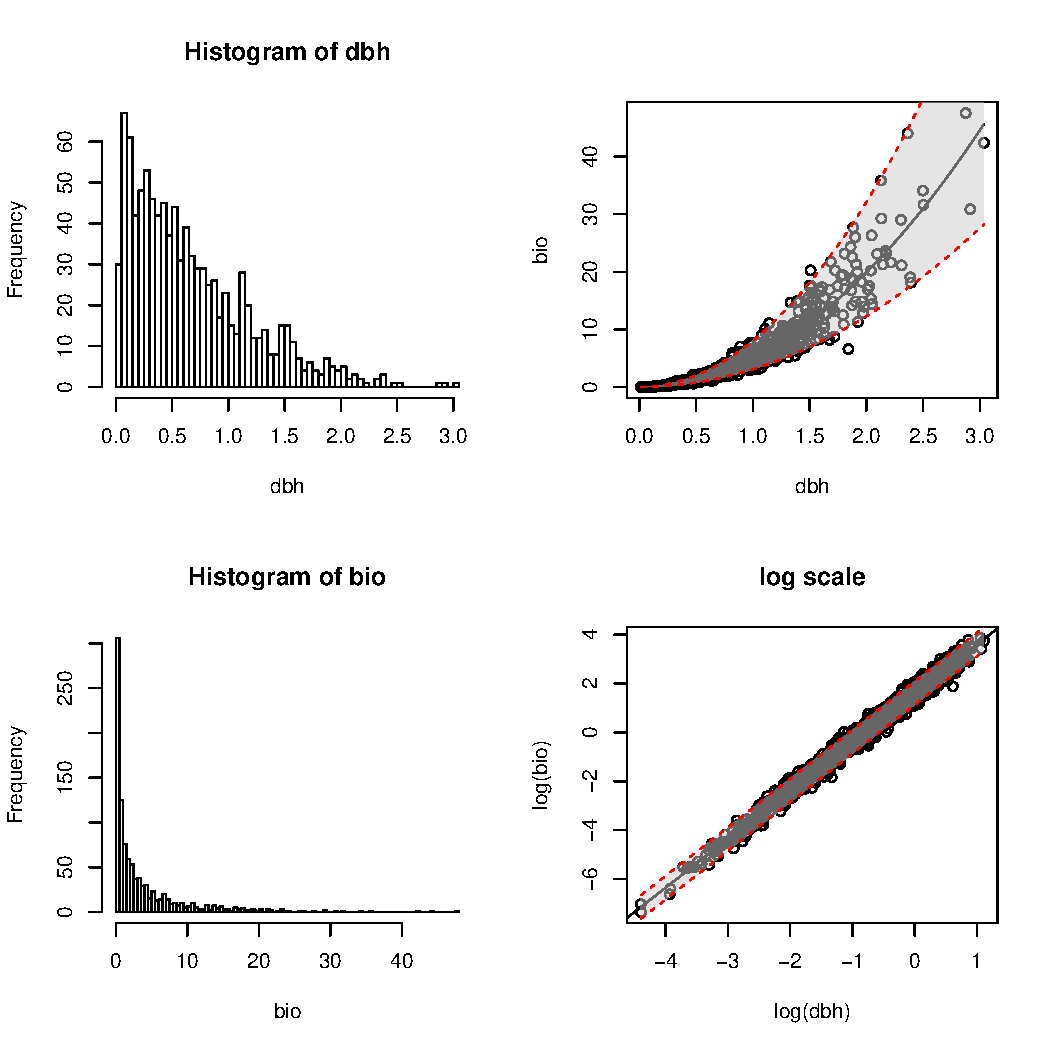
\includegraphics[scale = 0.25]{dbhModel}
  \end{figure}
\end{frame}
%
\begin{frame}
  \frametitle{The Model}
The allometric model is estimated by using ordinary least squares on the log-log model\\
  \begin{align}
  \label{2}
    \log(Y_i) & = \beta_0 + \beta_1 \log(X_i) + \epsilon
  \end{align}
  \begin{figure}
    \centering
    \caption{Plot of simulated log-allometric relationship typical of a sample plot (assumes one species only)}
    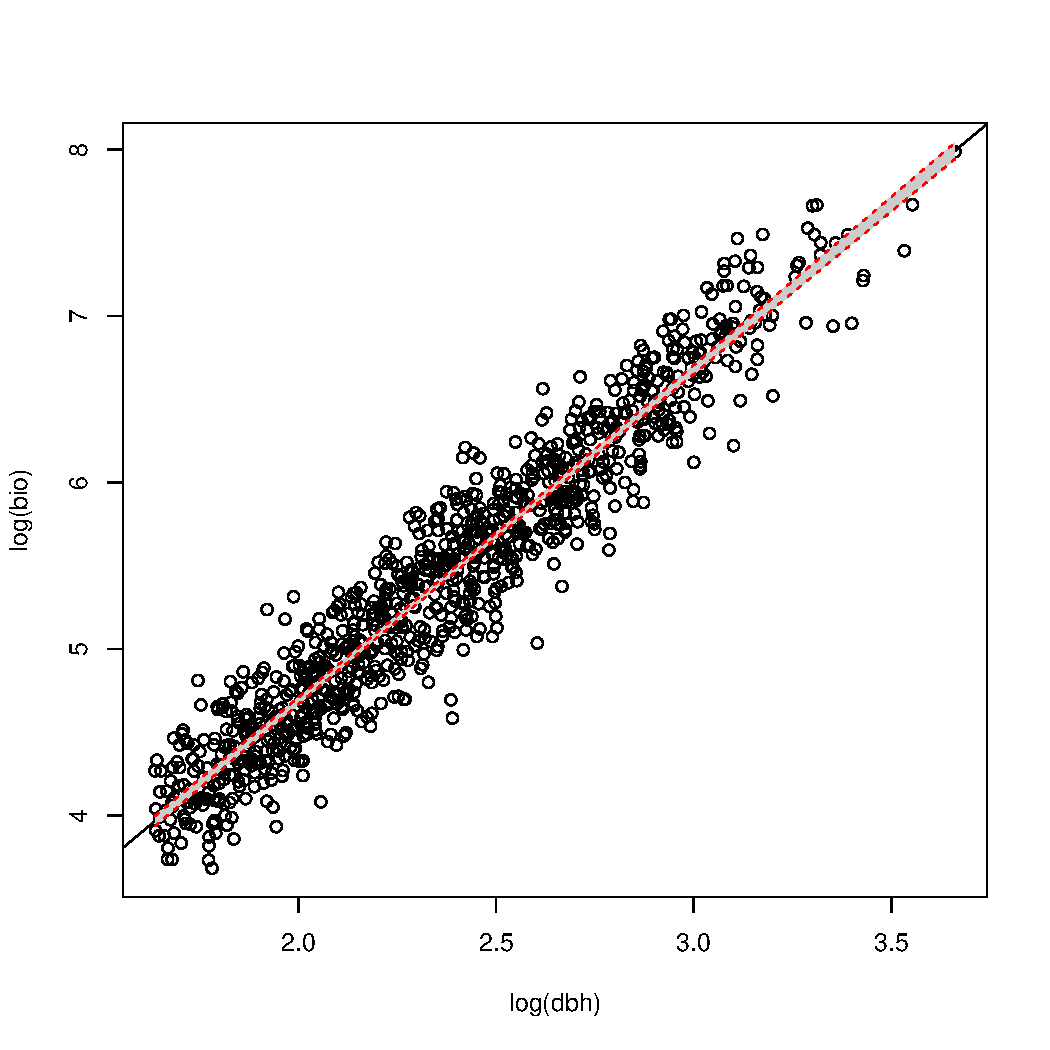
\includegraphics[scale = 0.15]{dbhLogModel}
  \end{figure}
\end{frame}
%
\begin{frame}
  Three questions:
  \begin{enumerate}
  \item What is the effect of sampling design on the estimate of total biomass and its variance estimator \vspace{3mm}
  \item What is the effect of sampling desing on the estimation of the coefficients $\beta_0$ and $\beta_1$ and the estimation of the variances associated with the coefficients $\beta_0$ and $\beta_1$ \vspace{3mm}
  \item How to optimize the sampling design for the desired sampling goals of stimating the total plot biomass with high precision while selecting large trees
  \end{enumerate}
\end{frame}
%
\begin{frame}
  \frametitle{Horvitz-Thompson Estimation}
  \section{Horvitz-Thompson Estimation}
  For a finite population with elements indexed by $i = 1, \ldots, N$ with a probability $\pi_i$ of being included in the sample $s$, the unbiased estimate of the population total is 
  \begin{align*}
    \hat{t}_y = \sum_{i \in s} \frac{y_i} {\pi_i}
  \end{align*}
\end{frame}

%%
%% Add in variance estimator and regression estimator
%%


%
% \section{Finite Population Design}
%   Consider a finite population of size $N$ derived from a continuous distribution. Denote this population $U = \{1, \ldots, N\}$. A simple and easy way to reduce variance in the estimation of a population total is the use of stratified sampling. Stratified sampling is accomplished by sampling from groupings of the ancillary variable $X$ known a priori. For instance, if the values of $X$ are grouped small, medium, and large, a stratified design consists of sampling $n_1$ elements form the small group, $n_2$ elements from the medium group, and $n_3$ elements from the large group. In general, this is extended to $h$ strata where the size of stratum $h$ is known and denoted $N_h$ and the population size is 
%   \begin{align*}
%     N & = \sum_{h = 1}^H N_h. 
%   \end{align*}
% The population total is
%   \begin{align*}
%     t_y & = \sum_{i \in U} y_i\\
%     & = \sum_{h = 1}^H t_h\\
%     & =\sum_{h = 1}^H N_h \bar{y}_h
%   \end{align*}
% where $t_h$ is the stratum total and $\bar{y}_h$ is the stratum mean. In stratified sampling, the $\pi$ estimator for the population total is 
%   \begin{align*}
%     \hat{t}_\pi & = \sum_{h = 1}^H \hat{t}_{h \pi}
%   \end{align*}
% where $\hat{t}_h$ is the $\pi$ estimator of $t_h$. The variance of the estimator $\hat{t}_\pi$ is given by
%   \begin{align*}
%     V(\hat{t}_\pi) & = \sum_{h = 1}^H V(\hat{t}_{h \pi})
%   \end{align*}
% where $V(\hat{t}_{h \pi})$ is the stratum variance of the stratum total $\hat{t}_{h \pi}$. An unbiased variance estimator for the stratified design is 
%   \begin{align*}
%     \hat{V}(\hat{t}_\pi) & = \sum_{h = 1}^H \hat{V}(\hat{t}_{h \pi})
%   \end{align*}
% where $V(\hat{t}_{h \pi})$ is the estimated stratum variance. Within each stratum $h$, a simple random sample of size $n_h$ can be taken. Under this design $s_h$ for sampling stratum $h$, the $\pi$ estimator for the population total $\sum_{i \in U} y_i$ is 
%   \begin{align*}
%     \hat{t}_{\pi} & = \sum_{h = 1}^H N_h \bar{\bm{y}}_{s_h}
%   \end{align*}
% where $\bar{\bm{y}}_{s_h} = \sum_{i \in s_h} \frac{y_i} {n_h}$ is the sample mean for stratum $h$. The variance for the estimator of the population total is 
%   \begin{align*}
%     V(\hat{t}_\pi) & = \sum_{h = 1}^H N_h^2 \frac{1 - f_h} {n_h} s^2_{y U_h}
%   \end{align*}
% where $f_h = \frac{n_h} {N_h}$ is the sampling fraction in stratum $h$ and 
%   \begin{align*}
%     s^2_{y U_h} = \frac{1} {N_h - 1} \sum_{i \in U_h} (y_i - \bar{y}_{U_h})^2    
%   \end{align*}
% is the stratum variance and $\bar{y}_{U_h} = \sum{i \in U_h} \frac{y_i} {N_h}$ is the stratum mean. An unbiased estimator of the variance is 
%   \begin{align*}
%     \hat{V}(\hat{t}_\pi) & = \sum_{h = 1}^H N_h^2 \frac{1 - f_h} {n_h} s^2_{y s_h}
%   \end{align*}
% where
%   \begin{align*}
%     s^2_{y s_h} = \frac{1} {n_h - 1} \sum_{i \in s_h} (y_i - \bar{y}_{s_h})^2
%   \end{align*}
% is the stratum variance in stratum $h$. The mean plot biomass can then be calcualted as $\frac{\hat{t}_\pi} {N}$ and the variance estimator for the mean plot biomass is $\frac{1} {N^2} \hat{V}(\hat{t}_\pi)$.
% 
%
\begin{frame}
  \section{Sampling Design}
  \begin{enumerate}
    \item Count (roughly estimate) the number of trees on the plot of interest in each stratum category of interest (e.g. small, medium large). \vspace{3mm}
    \item Based on the goals of the study, divide the sampling effort $n$ into the categories of interest, making sure to keep a minimum of 5? elements per stratum category.
  \end{enumerate}
\end{frame}
%
\begin{frame}
  \section{Estimation of the model}
  \begin{itemize}
    \item The log model can be estimated by using weighted least squares regression with the weight matrix $W = diag(\hat{\pi}_1, \ldots, \hat{\pi}_N)$ \vspace{3mm}
    \item The estimates then be transformed into by appropriately transforming the variance estimates through a Delta method like transformation.
  \end{itemize}
\end{frame}
%
\begin{frame}
  \section{Simulation and results}
%
  Six different sampling schemes were considered
  \begin{enumerate}
    \item Simple random sampling (SRS)
    \item Probability proportional to size sampling (PPS)
    \item Empirical cumulative distribution function (ECDF)
    \item Adaptive estimation of the PPS design (APPS)
    \item Adaptive estimation of the ECDF (AECDF)
    \item Stratified sampling with simple random sampling within each stratum (STSI)
  \end{enumerate}
\end{frame}
%
\begin{frame}
  Comapring the designs
  SRS sampling is the best known and one of the easiest sampling schemes to implement in the field as it only requires knowing (or estimating) the number of trees on the plot, but it fails to preferentially select large dbh trees and it is the basis for comparison for a reduction of variance so will not be efficient.
\end{frame}
%
\begin{frame}
  PPS sampling assigns sample inclusion probabilities based on a size variable known a priori, in our case we would use dbh if it was known. PPS sampling assigns sample weights for element $i$ of $\pi_i = \frac{x_i} {\sum_{i \in U} x_i}$. This presents problems for implementation in the field as it requires measuring all of the dbh values on the plot and labeling the trees. This labeling could be done in practice, but might be prohibitive in cost of time but will be highly efficient, in fact this scheme will reduce variance estimates more than any other method under the proposed model \eqref{1}. PPS sampling will also preferentially sample larger dbh trees relative to smaller dbh trees. PPS sampling meets criteria one and two but not three.\\
  ECDF sampling assigns sample inclusion probabilities based on the finite population empirical distribution function $F(\cdot)$ where $F(x_{(n)}) = \frac{n} {N}$ for $x_{(n)}$ the $n^{th}$ order statistic. Like PPS sampling, this requires knowing the values of the dbh a priori, which is not possible in this particular example. The ECDF sampling design does provide a point of comparison of the AECDF method as the ECDF is a best case scenario of the AECDF method (i.e. if the ECDF method is not sufficient for this problem, then the AECDF design is necessarily not sufficient). The ECDF method will reduce the variance relative to SRS and will preferentially sample larger trees, thus meeting criteria one and two but not three.
\end{frame}
%
\begin{frame}
  STSI sampling assigns sample inclusion probabilities for different size classes according to a simple random sampling scheme. Stratified sampling has the advantage of grouping similar elements of the population and thus reducing the variance of estimates by reducing within group variances. STSI sampling can also be made to preferentially sample larger trees by preferentially sampling the largest dbh class. STSI sampling can easily be implemented in field by initially estimating the number of trees in each size class on the plot and then using a random number generator in a tablet PC or smartphone to randomly select the sample within each size class. The STSI meets all three of the design criteria of interest and its performance relative to other designs is of interest.\\
  AECDF sampling assigns sample inclusion probabilities adaptively so that in the superpopultion model asymptotics the design is equivalent to ECDF sampling. AECDF sampling has the advantage in that it can be easily implemented in the field using modern technology like a tablet computer and excel spreadsheet. At each tree dbh measurement, a up/down sampling decision can be made and in the superpopulation model these sampling decisions approximate ECDF sampling without knowing a priori the values of dbh. AECDF also preferentially samples larger dbh trees. For finite populations, the question of interest is the effect of the AECDF design on the estimation of plot level biomass. The AECDF design meets criteria one and three, and the effect of this design on criteria two is of interest.
\end{frame}
%
\begin{frame}
  Using simulated data for dbh and biomass as shown in Figures 1-3 as a finite population approximating the true population criteria two can be evaluated for the different designs. From Table 1, it is seen that the most efficient design is PPS sampling with a relative efficiency of 0.12 for this particular simulation. The ECDF and STSI designs perform relatively similarily with respect to the relative efficiency measure with the STSI design being easier to implement without prior knowledge of the distribution of dbh. The AECDF method has relative efficiency higher than SRS and would only be useful if design criterions one and three are of interest.\\
\end{frame}
%
\begin{frame}
  % latex table generated in R 3.0.2 by xtable 1.7-1 package
  % Tue Jan 28 14:38:53 2014
  \begin{table}
    \centering
    \caption{Bias and Variance for design based estimates of mean plot biomass}
    \begin{tabular}{rrr}
    \hline
    & Bias & Relative Efficiency \\ 
    \hline
    SRS & -0.00 & 1.00 \\ 
    ECDF & -0.02 & 0.67 \\ 
    PPS & -0.10 & 0.12 \\ 
    AECDF & 0.00 & 1.35 \\ 
    STSI & -0.00 & 0.59 \\ 
     \hline
  \end{tabular}
  \end{table}
\end{frame}
%
\begin{frame}
  \section{Appendix - Current discussion items, thoughts, hypotheses, and other trains of thought}
  \begin{itemize}
    \item First, we need to pin down the primary questions of interest and define the goals
    \begin{itemize}
      \item Is the goal to sample large trees that will likely have a longer chronology and thus allow a better back forecast of biomass in a probabilistic way?
      \item Is the goal to decrease the uncertainty about biomass for large values of dbh?
      \item Is the goal to develop an adaptive sampling design that can be implemented in field to preferentially select larger trees in a statistically sound way while maintaining a probabilistic sample or is it to design a robust sampling design that is easy to implement?
    \end{itemize}
    \item Does the design need to incorporate multiple species? perhaps you could stratify based on size and species?
  \end{itemize}
\end{frame}
%
\end{document}